\onecolumn
\section{Manual analysis}\label{app:man_analysis}

Our quantitative tests provide information on when a model behaves locally and when globally in automated form but they do not consider whether that behaviour is incorrect or not.
More simply put, we do not know whether the changes that we observe are actually resulting in incorrect translations.
We complement these scores with an elaborate manual analysis, which provides more insight into the nature of the non-compositional behaviour we registered.

\subsection{Setup}

\paragraph{Data sampling} We randomly sample 900 examples for substitutivity (100 for each \{model\}$\times$\{test data type\} tuple) and 900 examples for systematicity (50 for each \{model\}$\times$\{test data type\}$\times$\{S$_1^\prime$, S$_3$\} tuple), randomly distributed over templates.
In all cases, we sample sentences randomly from the five seeds that we trained, and from all templates.
For substitutivity, we sample five examples for each synonym for every \{model\}$\times$\{test data type\} pair.

\paragraph{Annotation procedure}
For each of these samples, we annotate how they differ, where we distinguish between four general categories:
\begin{itemize}[noitemsep,topsep=0pt]
\item[i.] \emph{Rephrasing}: part of the sentence is rephrased (but both phrases are equally (in)correct);
\item[ii.] \emph{Source ambiguities}: there is an ambiguity in the source sentence, and the model switches its interpretation; 
\item[iii.] \emph{Errors}: one of the translations contains an error that the other one does not;
\item[iv.] \emph{Formatting}: minor formatting changes, consisting mostly of insertions/deletions of punctuation.
\end{itemize}

\noindent For the substitutivity data, we separately annotate changes that are related to the translation of the synonym, where we distinguish cases in which both synonyms are correctly or incorrectly translated from cases in which one of the translations is correct.
We annotate all changes observed in a sample -- one sentence may thus contain annotations for multiple changes -- and report the relative frequency of each class of errors.

\begin{figure}[h]\centering
\begin{subfigure}[b]{0.25\textwidth}
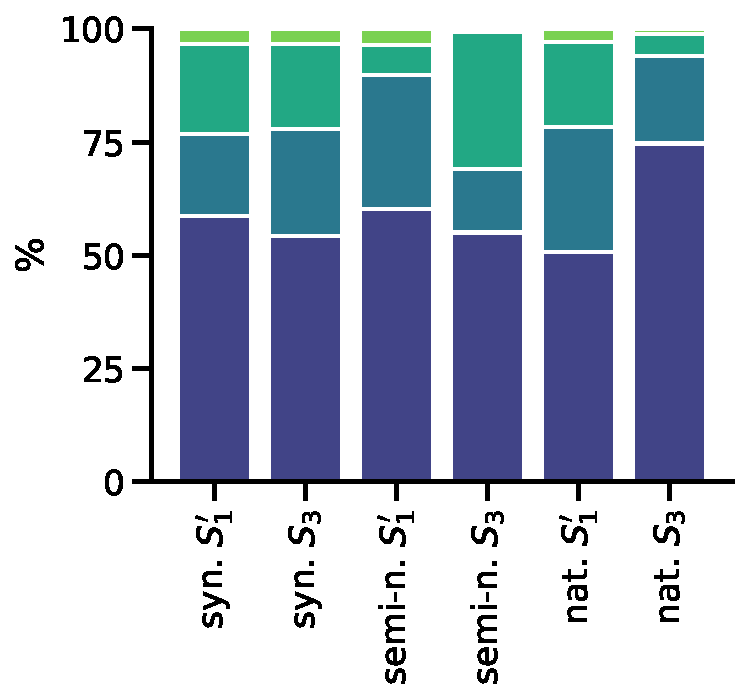
\includegraphics[width=\textwidth]{figures/analysis_appendix/systematicity_small.pdf}
\caption{Small training set}
\end{subfigure}
\begin{subfigure}[b]{0.25\textwidth}
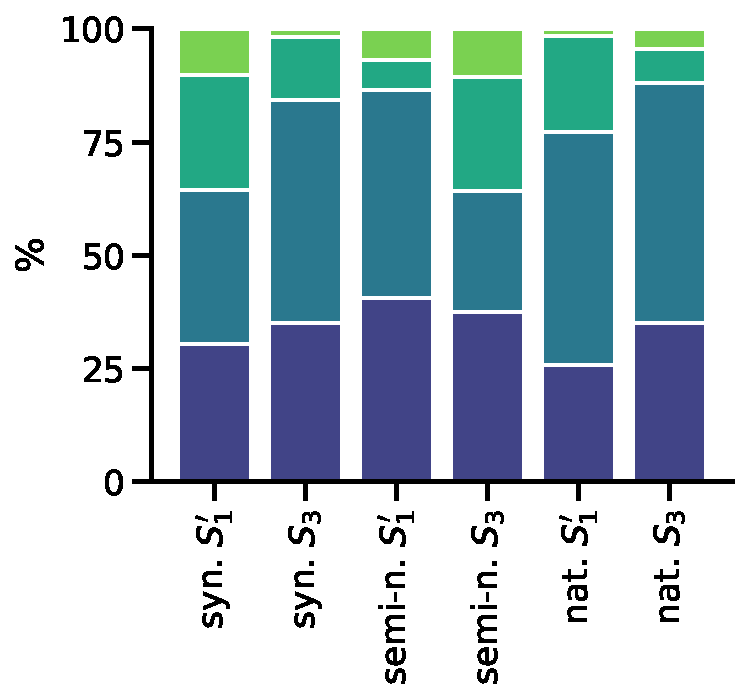
\includegraphics[width=\textwidth]{figures/analysis_appendix/systematicity_medium.pdf}
\caption{Medium training set}
\end{subfigure}
\begin{subfigure}[b]{0.41\textwidth}
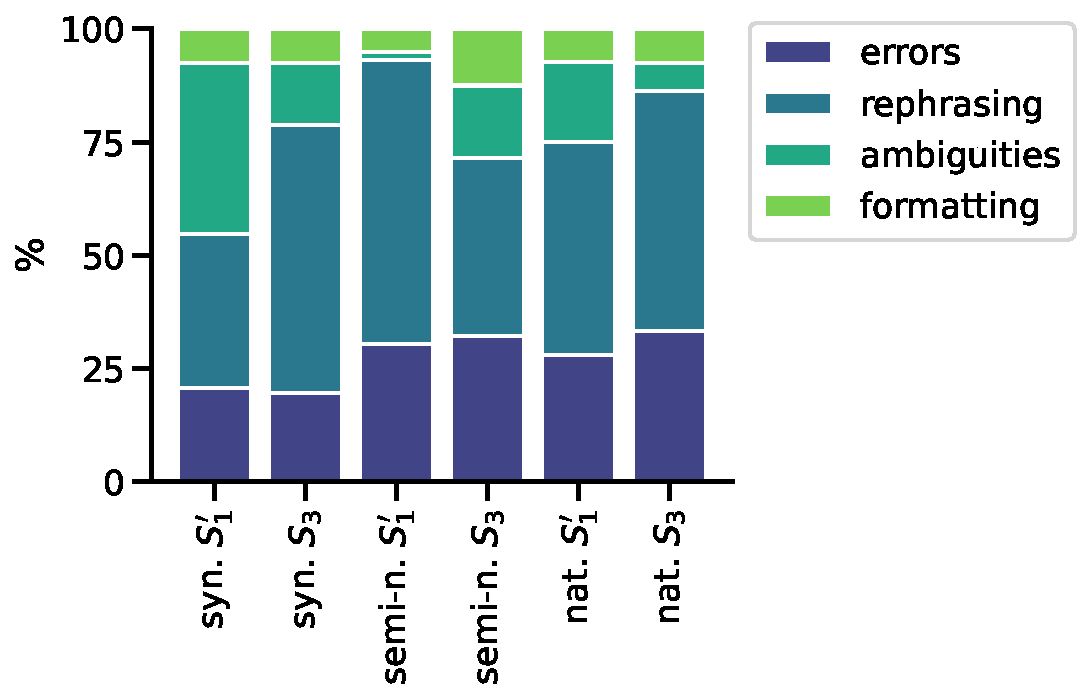
\includegraphics[width=0.9\textwidth]{figures/analysis_appendix/systematicity_full.pdf}
\caption{Full training set}
\end{subfigure}
\caption{Distribution of error types for sentences that contain inconsistencies in systematicity, detailed per model trained on the training set sizes in the subcaptions.}
\label{fig:ap_systematicity_analysis}
\end{figure}
\begin{figure}[t]\centering
\begin{subfigure}[b]{0.22\textwidth}\centering
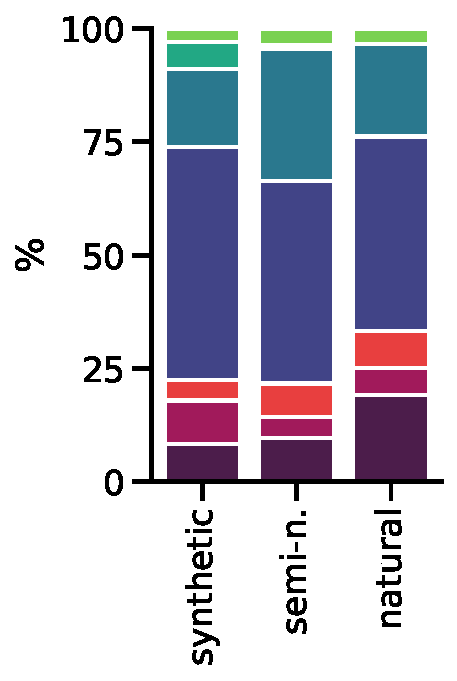
\includegraphics[width=0.79\textwidth]{figures/analysis_appendix/substitutivity_small.pdf}
\caption{Small training set}
\end{subfigure}
\begin{subfigure}[b]{0.22\textwidth}\centering
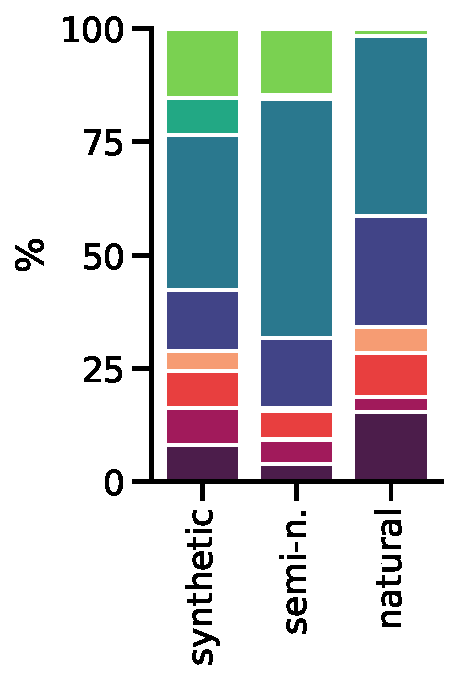
\includegraphics[width=0.79\textwidth]{figures/analysis_appendix/substitutivity_medium.pdf}
\caption{Medium training set}
\end{subfigure}
\begin{subfigure}[b]{0.43\textwidth}\centering
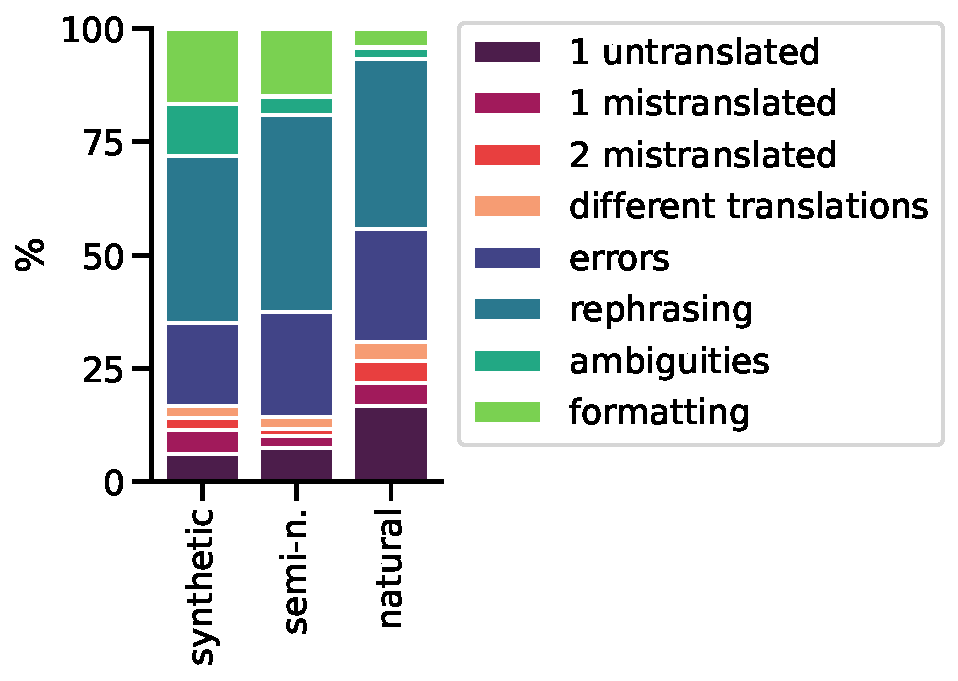
\includegraphics[width=0.85\textwidth]{figures/analysis_appendix/substitutivity_full.pdf}
\caption{Full training set}
\end{subfigure}
\caption{Distribution of the types of inconsistencies observed in the substitutivity test, detailed per model trained on the training set sizes in the subcaptions.
The red colour scheme represents error types specific to this experiment.}
\label{fig:ap_substitutivity_analysis}
\vspace{-.3cm}
\end{figure}

\subsection{Results}

We provide a summary of the results in Figure~\ref{fig:ap_systematicity_analysis} for systematicity and Figure~\ref{fig:ap_substitutivity_analysis} for substitutivity.
As a general trend, the results reflect that in models trained on smaller datasets, more mistakes are actually errors, rather than multiple correct alternatives.
In the systematicity test, 59\% of the inconsistencies for the models trained on the smallest dataset are erroneous changes, versus 34\% and 27\% in the models trained on the medium and largest dataset,
when we average the percentages over the different subsets annotated.
For substitutivity, the percentage of erroneous changes unrelated to the synonyms comprises 46\%, 18\% and 22\% for the smallest, medium and full dataset, respectively.
On top of that, there were inconsistencies related to the synonyms, that represented 26\%, 26\% and 21\% for the three dataset sizes, respectively.
While this is expected, to some extent, it still constitutes a problem: for models trained on smaller amounts of data, being able to translate in a compositional manner is particularly relevant.
Below, we further elaborate on the types of inconsistencies encountered per annotation category, including some examples.

\subsubsection{Rephrasing}
A large portion of the inconsistencies concerns pairs where one translation can be considered a rephrased version of the other translation.
A common cause of this is a \textbf{reordering of words} that does not impact the grammaticality or meaning of the Dutch sentence -- e.g.\ in sentences with adverbs (\exa{heeft de burgemeester zeker in de gaten} vs \exa{heeft zeker de burgemeester in de gaten}) or relative clauses with direct objects (\exa{die genieten van de vakantie} vs \exa{die van de vakantie genieten}).
We could not trace these reorderings back to the specific change made in the systematicity or substitutivity tests.
Consider, for instance, Example \ref{ex:zeker}, where the reordering happens as a consequence of changing the word \exa{king} to \exa{father}.
Note also that while these translations both contain an error (\exa{neemt \dots in de gaten}), this is not marked as an inconsistency, because it is shared between the translations.

\ex.\label{ex:zeker}
\a. \textsc{EN}: The aunts criticise the \{king, father\}, and the man definitely observes the mayor.
\b. \textsc{NL}: (\dots) en de man neemt zeker de burgemeester in de gaten.
\c. \textsc{NL}: (\dots) en de man neemt de burgemeester zeker in de gaten.


Another commonly occurring case of rephrasing is one where the two translations include terms that are (nearly) \textbf{synonymous terms} in Dutch.
Some examples are the translation of athlete (\exa{sporter} vs \exa{atleet}), wish (\exa{wensen} vs \exa{willen}) and observe (\exa{observeren} vs \exa{waarnemen}).
Some of them can appear in the same context but for others the two words would typically appear in different types of texts.
For instance, the word \exa{dokter} is used in more informal contexts than the word \exa{arts} (both translations of \exa{doctor}).
Again, we could not identify an interpretable pattern for when the model emits one instead of the other -- they were not understandably related to the modifications we made to the inputs.

\subsubsection{Source ambiguities}
An intriguing category that we had not anticipated were cases in which the source sentence contained ambiguities, such as \textbf{polysemous words} %whose translation in Dutch is not polysemous 
(e.g.\ \exa{director} translated to \exa{directeur}, referring to the director of a company, and \exa{regisseur}, indicating the director of a movie).
Other ambiguities encountered were \textbf{scope ambiguities}, that were particularly prominent for the systematicity test.
In that test, we concatenate two sentences, and the ambiguity was often related to the verb in the first sentence -- e.g.\ in Example~\ref{ex:director}: 

\ex.\label{ex:director}
\a. \textsc{EN}: The friend wishes that the \{lawyers, directors\} scream, and the victims (\dots)

While we intended this to be a conjunction of two independent sentences, there is also a reading where \exa{wishes} takes scope over the entire second conjunct.
In Dutch, those two cases are distinguishable because they trigger a different word order in the embedded clause (SOV), which is not grammatical for main clauses.
Such scope changes often lead to very questionable interpretations of the English sentence, as is the case for Example~\ref{ex:2CV}:

\ex.\label{ex:2CV}
\a. \textsc{EN}: The victims want that the \{doctors, mayors\} run, and the victims read an article about the case of a procedure which includes a repayment plan.
\b. \textsc{EN}: The farmers think that the \{butchers, mothers\} laugh, and an error can only be seen whenever we have a basic plan that is constantly compared to our real actions.
\c. \textsc{EN}: The women wish that the \{painters, victims\} walk consciously, and every 2CV or Dyane can basically be used as a donor.

Interestingly, the models sometimes also changed the order in the relative clause when a scope change was not possible, for instance when the second conjunct was a question, or the verb in the first sentence did not allow to take scope over the second conjunct without the presence of the word \exa{that}.
See Example~\ref{ex:vaders_president}. We underline the incorrect part of the translation, here and in erroneous examples that follow.

\ex. \label{ex:vaders_president}
\a. \textsc{EN}: The victim observes the \{leader, king\}, and the fathers carefully avoid the president.
\b. \textsc{NL}: Het slachtoffer observeert de leider en de vaders \underline{de president zorgvuldig vermijden}.
\c. \textsc{NL}: Het slachtoffer observeert de koning en de vaders vermijden voorzichtig de president.

These examples indicate that the interpretation of scope change might not be applicable here and that instead, the model is applying some heuristic where particular words trigger a relative clause order.

\subsubsection{Target errors}
In the category `target errors', some of the errors can be easily traced to individual words, whereas others indicate overall misinterpretations of the input.

\paragraph{Single word errors}
Errors that consist of single words are caused by words that are either missing, wrongly translated or untranslated.
Changes due to \textbf{missing words} can be very minor but nevertheless render one of the sentences ungrammatical (e.g.\ \exa{De tante achter de truck bewonderde de directeur}, correct, vs \exa{De tante achter de truck bewonderde directeur}, incorrect),
or yield grammatical sentences that have a slightly different meaning (e.g.\ \exa{de arts die yoghurt eet} vs \exa{de arts die \emph{de} yoghurt eet}).
Missing words can also render translations both ungrammatical and semantically incorrect, which occurred mostly in case of missing nouns or verbs (e.g. \exa{de bakker die ons herkent, merkt de koning op}, correct, vs \exa{de bakker die ons de koning herkent}, incorrect).

We also encountered pairs where one translation contained \textbf{untranslated source words}.
This happened with some of the words in our synthetic templates (e.g. \exa{ooms}/\exa{uncles}, \exa{butchers}/\exa{slagers}) but also with words from the natural sentences (e.g.\ \exa{extrusion}/\exa{extrusie}, \exa{soils}/\exa{bodem}).
These cases mark examples where local processing would have been helpful to the model: as evidenced by the alternative translation in the pair, the model does have access to the correct translation.

Thirdly, we observed cases of \textbf{mistranslated words}, where words unrelated to the change locus received a wrong translation in one of the two sentences but a correct one in the other, for example:
	\exa{poets} being translated as \exa{dichters} (correct) vs \exa{de potten} (incorrect), \exa{general} as \exa{generaal} (correct) vs \exa{wandeling} (incorrect), or \exa{productform} as \exa{productvorm} (correct) vs \exa{productformulier} (incorrect).

\paragraph{Multi-word errors} Other types of errors are less easily located to individual words but indicate an overall misinterpretation of the input, such as the \textbf{change in the tense} as displayed in Example~\ref{ex:musicians},
and the \textbf{change in agreement} displayed in Example~\ref{ex:begrijpen}.
In these particular cases, the source of confusion is explainable: in the first case, the model is combining a present tense verb with a word-order that does not support that, even though such a word order does exist (\exa{in het najaar van 2005 \dots en komen er al snel een paar \dots}).
In the second case, \exa{begrijpen} should agree with \exa{schilder} but instead agrees with the word \exa{doctors}, much earlier in the sentence.
In both of these cases, a more locally compositional approach to translating would have yielded correct translations.

\ex. \label{ex:musicians}
\a. \textsc{EN}: (\dots) and in autumn 2005, five musicians join their forces and soon a couple of potential songs came into being in the rehearsal room.
\b. \textsc{NL}: (\dots) in het najaar van 2005 voegen vijf muzikanten zich bij hun krachten en al snel kwamen er een paar potentiële nummers in de oefenruimte.
\c. \textsc{NL}: (\dots) in het najaar van 2005 bundelen vijf muzikanten hun krachten en al snel \underline{komen} er een paar potentiële nummers tot stand in de oefenruimte.


\ex. \label{ex:begrijpen}
\a. \textsc{EN}: The doctors that laugh admire the \{president, baker\}, the painter that admires her understands the king.
\b. \textsc{NL}: (\dots) de schilder die haar bewondert, \underline{begrijpen} de koning.
\c. \textsc{NL}: (\dots) de schilder die haar bewondert begrijpt de koning.

Finally, we would like to point out an error type that relates to the \textbf{semantic role assigned to agents}, and brings about a lot of other changes in the process.
For instance, in Example~\ref{ex:father}, \exa{the fathers} is removed from the main clause and moved into the relative clause, leaving the main clause without its direct object.

\ex. \label{ex:father}
\a. \textsc{EN}: The group of painters behind the truck forgets the \{president, friend\} and an article about the previous EESC Opinion on alcohol related harm, which looked at f, is read by the fathers
\b. \textsc{NL}: (\dots) en een artikel over het eerdere advies van het EESC over alcoholgerelateerde schade, \underline{die door de vaders wordt onderzocht, wordt gelezen}.
\c. \textsc{NL}: (\dots) en een artikel over het eerdere advies van het EESC over alcoholgerelateerde schade, die naar f uitkeek, wordt door de vaders gelezen.

\subsubsection{Formatting}

We marked inconsistencies as formatting changes if they were related to punctuation, capitalisation, hyphenation or differences in usage of spaces. 
In most cases, those cases were caused by commas: in one translation, a relative clause or two conjuncts were separated by a comma, whereas in the other translation the comma was left out.
In the cases that were caused by spaces (\exa{tumormassa} vs \exa{tumor massa}), there is a slight difference in correctness: in Dutch, compound nouns are not separated by spaces. 
Given how minor these mistakes are, we did not mark them as errors.
Example~\ref{ex:begrijpen} above provides an example for inconsistent usage of commas.
Formatting changes are far from the most frequent but they do become more prominent in models trained on larger training corpora.

\subsubsection{Inconsistencies in synonym translations}

The synonym errors are subdivided into cases where synonyms are simply translated differently (we observed this mostly for the models with larger training set sizes), cases where both translations were incorrect, cases in which only one translation is wrong, and cases in which one synonym was not translated but directly copied from the source.
Sometimes, the changes were quite peculiar, to give some examples from our natural corpus:

\ex.
\a. \textsc{EN}: The child admires the king that eats the \{doughnut, donut\}.
\b. \textsc{NL}: Het kind bewondert de koning die de donut eet.
\c. \textsc{NL}: Het kind bewondert de koning die de \underline{ezel} eet.

\ex.
\a. \textsc{EN}: - Yeah, a barbecue sauce \{moustache, mustache\} contest.
\b. \textsc{NL}: - Ja, een barbecue \underline{[missing `sauce']} met snor.
\c. \textsc{NL}: - Ja, een barbeceu saus snor wedstrijd.

How often each of these errors occur depends on the synonym.
Where some synonyms are more prone to being untranslated (like \exa{ladybird} and \exa{flautist}), some simply received many different correct translations (like \exa{shopping trolley}) yet others received errors very specific to the synonym (like \exa{eggplant} being translated as \exa{egg}$+$\exa{plant}, an interesting case because it reflects processing that is too local).
It should be noted that for all synonyms -- apart from the model with the small training dataset that cannot translate \exa{flautist} and \exa{ladybug} -- we have observed correct translations, indicating that the models did in fact acquire their meaning.

Further, it should be noted that while our substitutivity experiment provides insight into how the model copes with individual synonyms, the majority of the inconsistencies observed were still common target errors, rephrasings, changes in formatting or the result of source-side ambiguities. 
It is vital here to stress that the types of rephrasings, however, did not appear related to the writing style of the sentence. For instance, considering that the synonym changes were related to British and American spelling, and occassionally changed the tone of the sentence (e.g.\ \exa{aeroplane} could be considered more archaic compared to \exa{airplane}), one could anticipate changes in word choice in Dutch reflecting this change of style. However, the inconsistencies were virtually indistinguishable from those annotated for systematicity.